\chapter{Theory}\label{cpt:theory}
%Write about all the concepts which are used in the work to address the research questions and are key to understanding your work.

\section{Machine Learning}

\subsection{Introduction}

Machine learning is a subfield of artificial intelligence consisting of algorithms that makes computers able to learn to solve problems from data, in contrast to being programmed directly. Artificial intelligence is a wider field about making computers solve complex problems. Machine learning methods are often useful when it is difficult to create explicit models, unlike for example expert systems using handcrafted rules. Machine learning has become ubiquitous in modern computing with the rise of the internet and larger datasets that allows more sophisticated models to be trained. They are used for many different types of problems, some examples include email spam filtering, recommendation systems for online stores, internet search engines, vision systems for autonomous vehicles, chatbots and playing games like chess.

Machine learning was first named by Arthur Samuel in 1959 \cite{samuel59} when he developed a learning algorithm that made a computer able to play the game of checkers. The system consisted of a minimax search algorithm combined with a learned evaluation function. The evaluation function was a linear combination of manually defined board parameters with adjustable weights, where the weights were updated after a win or a loss.

An even earlier example of a machine learning algorithm was developed by Frank Rosenblatt in 1957 \cite{rosenblatt57}. He created a model known as the perceptron, that performed binary classification. It was inspired by the computational model of biological neurons from McCulloch and Pitts from 1943 \cite{pitts43}, which formulated that biological neural networks are able to learn things by adjusting the connection strength between the neurons in the network. Rosenblatt's perceptron consisted of multiple input neurons connected to one output neuron, where each connection had an associated weight that could be updated from training data. It also had a nonlinear activation function that worked as a thresholding mechanism.

\begin{figure}[H]
    \centering
    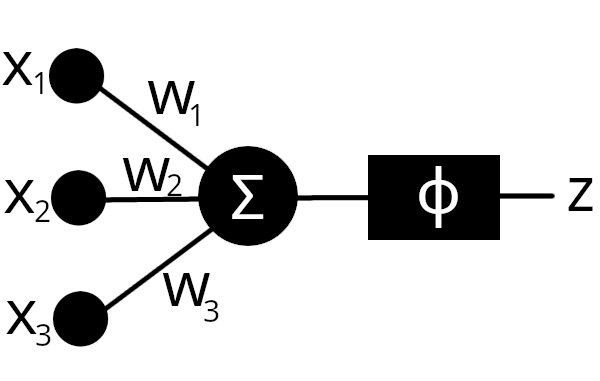
\includegraphics[width=0.8\linewidth]{Figures/Misc/Perceptron.png}
    \caption{Visualization of a perceptron model.}
    \label{fig:perceptron}
\end{figure}

In 1969 the influential book called Perceptrons by Minsky and Papert\cite{perceptronsbook} showed mathematically that the perceptron model was severely limited in what functions could be represented. The conclusion was that the data had to be possible to linearly separate, which essentially means that it must be possible to place a hyperplane in between the datapoints. The XOR function is a simple example of a function that is not linearly separable. The solution to learn such problems was to add additional layers of neurons with weights prior to the input layer, resulting in the model known as the Multi-Layered Perceptron (MLP). The backpropagation algorithm developed by Rumelhart, Hinton and Williams in 1986 \cite{backprop86} made it possible to train MLPs using gradient descent type algorithms commonly used in numerical optimization problems.

\subsection{Overview}

Machine learning consists of three fundamental components. The first is the dataset which is essential to properly learn the desired task. More recently the emphasis on better quality data combined with higher quantities has proven to be more efficient instead of coming up with new learning algorithms or models. The second component is the model, which is a mathematical equation that describes how to apply the data in order to make use of it. The model can also contain a set of learnable parameters. The final component is the learning algorithm that describes how the model with parameters is changed when training on the data.

One of the most widely used rigorous definitions of machine learning is the one from Tom Mitchell \cite{mitchellmachinelearning}. It states: ``A computer program is said to learn from experience E with respect to some class of tasks T and performance measure P, if its performance at tasks in T, as measured by P, improves with experience E.''

It is common to separate machine learning into three smaller categories depending on how the learning is done, which are called supervised learning, unsupervised learning and reinforcement learning. Supervised learning might be the most commonly applicable type of machine learning and consists of problems where the goal is to learn a mapping from an input to an output. This is achieved by training on a dataset containing both input data and corresponding labels or target values. The two main types of supervised learning are called regression and classification. Regression is what happens when the input data maps continuously to some output values and the goal is to approximate the underlying function. Classification is what happens when the output values have a discrete and finite domain, and while it might look like a discrete version of regression it will often rely on different types of learning algorithms. A typical regression problem can be to predict some value based on previously collected values, for example in predicting stock prices in finance based on historical data. A typical classification problem can be to determine what class a certain input belongs to, for example detecting fraudulent bank transactions automatically.

Unsupervised learning is about learning things from data without any labels or target values. There can be multiple goals with learning unsupervised. Some of the most common applications are trying to find patterns and structures in the underlying dataset through for example a clustering algorithm like k-means. Another application is to learn better representations or features of the data, for example for the purposes of dimensionality reduction and data compression through Principal Component Analysis (PCA), or as input to another learning algorithm often through autoencoders. The last example of using unsupervised features as input is particularly useful when the dataset is partially labeled, meaning only some of the input data has corresponding labels in what is called semi-supervised learning. The concept of features learned in an unsupervised way is also highly applicable to generative models for both text \cite{gpt3} and images \cite{stablediffusion} as it is often easier for a model to train on features already determined by another model. The compressed feature space is in this case often called a latent space. In comparison, training generative image models directly on raw pixel values can often make the training process significantly longer and more expensive in terms of compute.

The final category of reinforcement learning deals with problems where the goal is to train an agent to interact with an environment in order to accomplish specific tasks. It has a lot of overlap with control theory in its goals, as the environment and agent often can be modeled together as a dynamical system. The difference comes from that in reinforcement learning the input function is learned while it is often manually designed to meet certain requirements in control theory. According to Sutton, Barto and Williams \cite{rladaptivecontrol}, reinforcement learning can be interpreted as a form of direct adaptive optimal control. Optimal control means that the dynamical system together with its input satisfies some optimality conditions. Direct adaptive control means that the structure and parametric values of the controller input function is learned as an online problem. The way learning is done in reinforcement learning is by making the agent explore and experiment with certain degrees of randomness and getting rewards based on how capable it is of solving its designated tasks. The reward is then used to update the control law. One of the advantages of reinforcement learning over classical control theory is that it does not rely on creating models of the system first, which also means that it can be applied to many other types of systems. One of the first examples of playing games was TD-Gammon \cite{tdgammon} which used reinforcement learning to play backgammon. More recently, DeepMind used reinforcement learning with the MuZero model \cite{muzero} where it is able to both learn optimal strategies as well as the rules of the game, thus giving it the ability to play any game with enough training.

\subsection{Generalizability}

When training machine learning models it is desirable that they are able to generalize outside of the training data. This means that when presented with never before seen data the model should still provide reasonable outputs. For example would an email spam detection filter not be useful if it only was reliable on emails it had already seen. Generalizing outside the training data is what makes machine learning useful.

To measure how well a model generalizes it is common to split the dataset into two parts: a training set and a testing set. The training set is usually where most of the data ends up with something in the range of $60\%-80\%$ from the full set. The model is then trained exclusively on the training set while the performance is measured on both the training and testing sets. If the difference in performance measure is small it means that the model is able to generalize. However if the difference starts to increase it is said that the model overfits on the training data which makes it less generalizable.

Overfitting is something that often happens when the model is too complex in comparison to the underlying data distribution. It is also possible for a model to underfit, which can mean that the model is lacking in complexity to represent the data properly. In this case it will generally result in poor performance on both the training and testing set. When choosing models it is therefore desirable that they hit some sweet spot in between underfitting and overfitting. Determining aspects of the data generation process and making assumptions can then lead to more suitable models.

It is often desirable to train multiple different models and compare them against each other to get the best possible model. This could be entirely different types of models, models with different hyperparameters or models trained on separate data. Models often contain parameters which are predetermined instead of learned called hyperparameters which can influence the overall performance of the model. In order to properly compare models, the training set is often split again into a new smaller training set and a validation set. The validation set is then used for testing each model separately in order to compare them against each other, while the final testing set is used to get the actual generalizable performance of the selected model.

\subsection{Deep Learning}

Deep learning is a subfield inside the larger field of machine learning that is becoming increasingly popular in recent years. Whereas in classical machine learning it is more common to manually design the features that go into the models, deep learning instead relies on processing raw data and learning its own feature representations. The deep part of deep learning refers to how models usually have a hierarchy of abstraction levels for the learned feature representations, where the abstraction level of the features increases as the depth of the model increases. These features will build on the features learned from previous layers, which makes it possible to gradually build up complicated representations by increasing the model depth \cite{deeplearningbook}. A simple example could be to train a facial recognition model on images. In this case the shallow layers would learn features such as edges or specific colors, while the deeper layers would combine the edges and colors to create geometric objects followed by all the aspects needed to represent a face.

\begin{figure}[H]
    \centering
    \includesvg[height=10cm]{Figures/Misc/ann.svg}
    \caption{Visualization of a simple Fully-Connected Neural Network, represented as a directed graph.}
    \label{fig:ann}
\end{figure}

The Multi-Layered Perceptron is perhaps the simplest example of a deep learning based model, where each layer builds upon the output from the previous layers. Additionally, MLPs are also one of the simplest examples of Artificial Neural Networks (ANNs) and are often called Fully-Connected Neural Networks (FCNNs). FCNNs represent neural networks as multiple layers of nodes where each node in one layer is connected to every node in the subsequent layer. This allows for a compact representation of the forward pass using matrix multiplications denoting the connection strength between nodes. The general form of an FCNN can be expressed as:

\begin{equation}
    % multiline: without alignment
    % split: with alignment,
    \begin{split}
        \bm{z}_1 = & \bm{\phi_1}(\bm{W}_1 \bm{x} + \bm{b}_1) \\
        \bm{z}_2 = & \bm{\phi_2}(\bm{W}_1 \bm{z}_1 + \bm{b}_2) \\
        & \vdots \\
        \bm{z}_k = & \bm{\phi_k}(\bm{W}_k \bm{z}_{k-1} + \bm{b}_k)
    \end{split}
    \label{eq:ann_forward}
\end{equation}

\noindent with input $\bm{x} \in \mathbb{R}^N$, output $\bm{z}_k \in \mathbb{R}^M$ and intermediate hidden outputs $\bm{z}_i$. The weight matrices $\bm{W}_i$ and bias vectors $\bm{b}_i$ are learnable parameters of the neural network which transform the state layerwise. The $\bm{\phi}_i$ are called activation functions and are applied at the end of each layer in order to introduce nonlinearity in the function representation. Without nonlinear activation functions it would severely limit the representation capabilities of neural networks. Some common examples of activation functions include the sigmoid function: $\sigma(x) = \frac{1}{1 + e^{-x}}$, $\tanh(x)$ and the Rectified Linear Unit (ReLU): $\phi(x) = \max(x, 0)$. Many other types of activation functions also exist but what many have in common is that they are nonlinear and that they somehow restrict the input variables to some smaller domain. The choice of activation functions can be considered as hyperparameters and are chosen before the training process begins. Which activation function to use can often be dependent on the problem in order to exploit certain properties. Likewise, the number of layers and the number of hidden units are also hyperparameters determined before.

The universal approximation theorem \cite{Hornik1989MultilayerFN} states very simplified that neural networks are able to represent any mapping, assuming that the network is complex enough. Being complex enough is dependent on having a combination of enough layers to represent the given abstraction level, as well as having enough nodes at each layer to represent those specific features. Stated differently, this means that for any given problem there exists some network structure combined with a set of parameter values that can represent the desired mapping up to a given approximation accuracy. However, this theorem does not give any method to discover that network.

Deep learning methods instead rely on solving a numerical optimization problem in order to fit the network to the data from the mapping. This optimization method does not guarantee that the network becomes perfectly accurate, but it does often work well in practice. To do this it is necessary to define an objective function for the optimization problem, usually called a loss function $\mathcal{L}$ in deep learning context. The choice of loss function is problem dependent and there exists many different types of loss functions used in practice. It also can be thought of as a hyperparameter during the training process, although it is not strictly a part of the final network and only used during training. For supervised learning problems the loss function will be a function of the training data labels $\bm{y}$ and the predicted network outputs $\bm{\hat{y}} = f(\bm{x})$ for corresponding input data $\bm{x}$. The neural network (\ref{eq:ann_forward}) is described simply as $f$. For example is the Mean Squared Error (MSE) loss function defined as: 

\begin{equation}
    \mathcal{L}(\bm{y}, \bm{\hat{y}}) = \frac{1}{M} \sum_{m=1}^{M} (y_m - \hat{y}_m)^2
\end{equation}

\noindent for a single datapoint $\bm{y} \in \mathbb{R}^M$. Computing the loss over a batch of training data is done by averaging the loss functions of each datapoint. The MSE loss function is very commonly used for regression problems where the goal is to learn a continuous mapping between input and output. For classification problems, the Cross Entropy loss function is one of the most widely used:

\begin{equation}
    \mathcal{L}(\bm{y}, \bm{\hat{y}}) = - \frac{1}{M} \sum_{m=1}^{M} y_m \ln{(\hat{y}_m)}
\end{equation}

\noindent using that there are $M$ different classes. This is usually accomplished by modeling the output labels as one-hot encoded vectors.

The deep learning optimization can then be stated simply as the unconstrained minimization problem:

\begin{equation}
    \min_{\bm{\theta}} \quad \mathcal{L}(\bm{y}, \bm{\hat{y}})
\end{equation}

\noindent where $\bm{\hat{y}} = \bm{f}(\bm{x}; \bm{\theta})$ for a training set with input points $\bm{x}$ and outputs $\bm{y}$. The neural network $\bm{f}$ is parametrized by $\bm{\theta}$ containing the weight matrices and bias vectors. The parameter vector $\bm{\theta}$ is usually very high-dimensional, which leads to a very non-convex loss landscape. In order to find the global minima it is therefore necessary to use global optimization methods, but this is rarely done in practice as it is too computationally expensive considering both the high amount of parameters and also higher amounts of training data. Instead it is more common to simply treat the problem as it was convex and use gradient descent based methods in order to find a local minima. The performance difference from different local minimas turns out to not necessarily be that important in practice. Higher order optimization methods are also generally not used, as the size of the Hessian matrix would make it too expensive in terms of both computations and memory.

A gradient descent algorithm in its simplest form are described as:

\begin{equation}
    \bm{\theta} \leftarrow \bm{\theta} - \alpha \nabla_{\bm{\theta}} \mathcal{L}
    \label{eq:sgd}
\end{equation}

\noindent where the step size $\alpha$, usually called the learning rate in deep learning, is yet another hyperparameter. In order to perform gradient descent it is therefore necessary to compute the gradients from the loss function to the parameters $\nabla_{\bm{\theta}} \mathcal{L}$.

\begin{figure}[H]
    \centering
    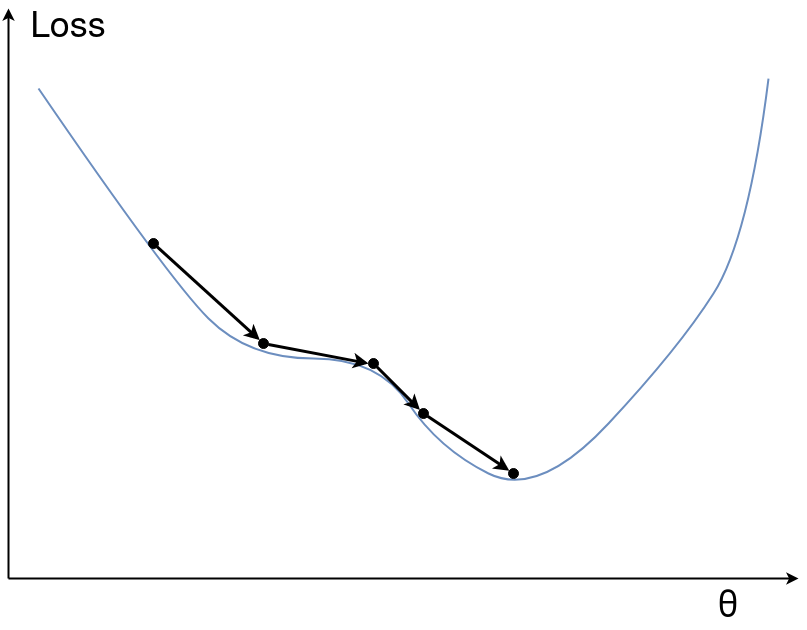
\includegraphics[width=0.8\linewidth]{Figures/Misc/gradientdescent.png}
    \caption{Simplified visualization of how gradient descent iteratively minimizes the loss function towards a local minima.}
    \label{fig:gradientdescent}
\end{figure}

Computing derivatives can be done in different ways. Symbolical gradient representations are generally too computationally expensive for deep neural networks, and numerical methods based on finite differences are too inaccurate to provide useful descent iterations. A middleground is to use automatic differentiation where individual expressions are done symbolically where each symbolic expression is evaluated numerically independent of the overall expression. Automatic differentiation is based on the chain rule from basic calculus where each expression is computed iteratively. It can be done in a forward or reverse mode that both results in the same output but depending on whether to start iterating from the input or the output. Forward mode is usually better if the resulting jacobian matrix is tall, meaning that the dimension of the input is smaller than the dimension of the output. Reverse mode is in contrast better for wide matrices where the input dimension is larger than the output dimension. As the goal is to compute gradients to the parameters of the neural network, reverse mode automatic differentiation will be significantly less expensive to compute. In deep learning context it is common to refer to reverse mode automatic differentiation as the backpropagation algorithm after it was independently re-discovered by the computer science community \cite{backprop86}.
 
For neural networks with multiple layers it is practical to compute gradients to the parameters of each layer separately. The gradients to previous layers can then be recursively computed based on the gradients to the inputs so far. To simplify notation, write $\nabla_{\bm{\theta}} \mathcal{L} = \frac{\partial \mathcal{L}}{\partial \bm{\theta}}$. Gradients to the parameters at layer $k$ are then given as:

\begin{equation}
    \frac{\partial \mathcal{L}}{\partial \bm{\theta}_k}
    = \frac{\partial \mathcal{L}}{\partial \bm{z}_k} \frac{\partial \bm{z}_k}{\partial \bm{\theta}_k}
    = \frac{\partial \mathcal{L}}{\partial \bm{z}_k} \frac{\partial \bm{\phi}_k}{\partial \bm{s}_k} \frac{\partial \bm{s}_k}{\partial \bm{\theta}_k}
\end{equation}

\noindent where $\bm{s}_k = \bm{W}_k \bm{z}_{k-1} + \bm{b}_k$. All the Jacobians above can be considered well-defined and easily computable analytically. For example will the jacobian $\frac{\partial \bm{\phi}_k}{\partial \bm{s}_k}$ be the derivative of the activation function which is implemented alongside the activation function. To get gradients to previous layers, apply the chain rule recursively:

\begin{equation}
    \frac{\partial \mathcal{L}}{\partial \bm{\theta}_{k-1}}
    = \frac{\partial \mathcal{L}}{\partial \bm{z}_k} \frac{\partial \bm{\phi}_k}{\partial \bm{s}_k} \frac{\partial \bm{s}_k}{\partial \bm{z}_{k-1}} \frac{\partial \bm{z}_{k-1}}{\partial \bm{\theta}_{k-1}}
    = \frac{\partial \mathcal{L}}{\partial \bm{z}_k} \frac{\partial \bm{\phi}_k}{\partial \bm{s}_k} \frac{\partial \bm{s}_k}{\partial \bm{z}_{k-1}} \frac{\partial \bm{\phi}_{k-1}}{\partial \bm{s}_{k-1}} \frac{\partial \bm{s}_{k-1}}{\partial \bm{\theta}_{k-1}}
\end{equation}

This generalizes to the recursive formula:

\begin{equation}
    \frac{\partial \mathcal{L}}{\partial \bm{\theta}_{i}}
    = \frac{\partial \mathcal{L}}{\partial \bm{z}_k} \frac{\partial \bm{z}_k}{\partial \bm{z}_{k-1}} \dots \frac{\partial \bm{z}_{i+1}}{\partial \bm{z}_i} \frac{\partial \bm{z}_i}{\partial \bm{\theta}_i}
\label{eq:backprop}
\end{equation}

\noindent with

\begin{equation}
\begin{aligned}[t]
    \frac{\partial \bm{z}_{i+1}}{\partial \bm{z}_i}
    = \frac{\partial \bm{\phi}_{i+1}}{\partial \bm{s}_{i+1}} \frac{\partial \bm{s}_{i+1}}{\partial \bm{z}_i}
\end{aligned}
\qquad
\qquad
\qquad
\begin{aligned}[t]
    \frac{\partial \bm{z}_i}{\partial \bm{\theta}_i}
    = \frac{\partial \bm{\phi}_i}{\partial \bm{s}_i} \frac{\partial \bm{s}_i}{\partial \bm{\theta}_i}
\end{aligned}
\end{equation}

\noindent which gives the complete backpropagation algorithm for neural networks. Computing gradients like this is also called to do a backward pass of the network.

\begin{figure}[H]
    \centering
    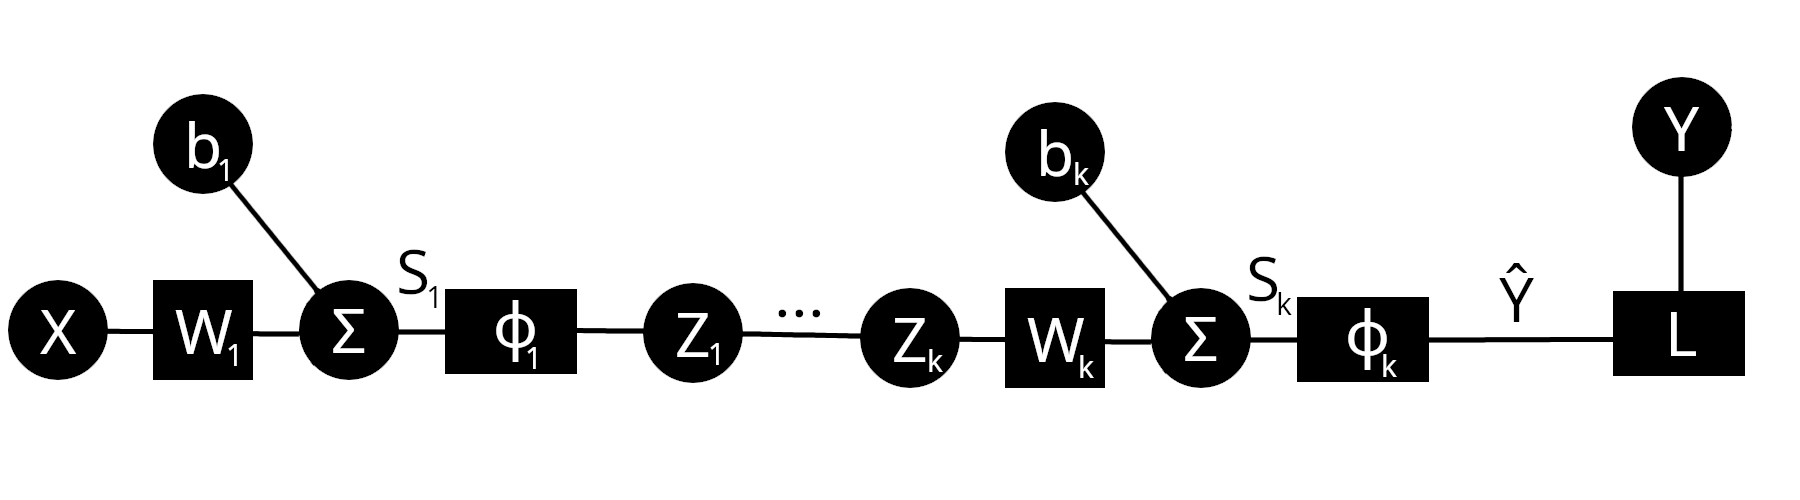
\includegraphics[width=0.8\linewidth]{Figures/Misc/deepnetwork.png}
    \caption{Visualization of a deep neural network.}
    \label{fig:deepnetwork}
\end{figure}

The current gradient descent algorithm will converge to the closest local minimum from the initial parameter values. There are some common techniques that can help to mitigate this somewhat and escape local minimas. As second order optimization methods are generally too expensive these techniques modify the gradient iterations themselves. A standard technique in deep learning is to use Stochastic Gradient Descent (SGD) instead of the normal gradient descent algorithm. The difference is that the stochastic version uses a subset of the training data called a minibatch at each update, compared to the whole data at once. The minibatches are drawn from random partitions of the training set, and it is common to re-randomize or shuffle the minibatch partitions after a full pass of the training data. SGD is particularly useful when dealing with large datasets for memory reasons, but the stochastic nature makes the loss landscape shift at each iteration, thus making it possible to escape local minimas. Another addition is to add momentum to the iterations so that the gradient updates can overcome short hurdles. Momentum is implemented in practice by averaging the current gradient with the $K$ previously computed gradients and using the averaged gradient as the actual descent direction. It can also result in faster convergence due to reducing oscillations in valleys in the loss landscape. A final technique to mention is that it is common to adjust the learning rate as the learning happens, usually with a larger learning rate at the beginning and then a smaller one towards the end. One of the most common optimizers currently used in deep learning is the Adam (Adaptive Momentum) optimizer \cite{kingma2017adam} using all of these features.

In some cases with smaller datasets it is possible to use approximate second order optimization methods. These are also called quasi-Newton methods due to using an approximation of the Hessian matrix, as computing the full Hessian matrix is not tractable. In deep learning context the most common method is the Limited-memory Broyden–Fletcher–Goldfarb–Shanno (L-BFGS) algorithm \cite{numericaloptimization}.

There are also multiple techniques to help deep neural networks generalize better and reduce overfitting. A common method is to add regularization on the network parameters, which effectively reduces the model complexity as the parameter values are driven close to zero. The strength of the regularization is a tunable hyperparameter and can be thought of as a tradeoff between model complexity and data fit after training. Dropout is another technique useful during training that makes it more difficult for networks to simply memorize the training data and instead forces them to learn better representations. This is done in practice by adding a random chance that every node in every layer is simply turned off for that training iteration. The probability is yet another hyperparameter. Dropout is also only used during training, and turned off when the network is used for inference.

To conclude the section on deep learning it is worth mentioning that there exists other types of ANNs than just FCNNs. Convolutional Neural Networks (CNNs) are very common when dealing with data that contains translationally invariant features \cite{deeplearningnature}. Images are the typical example of this, as training a CNN to classify objects in images means that the position of the object inside the image should not impact the classification. CNNS are inspired by linear FIR filters from digital signal processing and image processing, where an input signal sent through a filter results in an output of the mathematical convolution of the input signal and the filter impulse response. In classical image processing such filters were manually designed to detect certain features in images \cite{imageprocessing}, while more modern CNNs are basically learning their own filter representations. Using CNNs instead of FCNNs for image processing tasks will usually result in much fewer total network parameters.

Another type of ANN are Recurrent Neural Networks (RNNs) \cite{deeplearningnature}, which are intended for handling sequential data. Typical examples include time-series data, or text and natural language processing. They work by processing one element of the input sequence at a time and modifying an internal hidden state of the RNN containing the latent representation of the sequence. One problem with RNNs is that they heavily suffer from what is known as the vanishing gradient problem \cite{vanishinggradients}, which is also encountered for any deeper network. Due to the backpropagation algorithm recursively computing gradients, the gradient magnitudes have a tendency to shrink for each successive layer due to magnitudes smaller than 1 being multiplied together. The Long-Short Term Memory (LSTM) architecture is a modified RNN that solves the problem of vanishing gradients, and are in practice always preferred over standard RNNs. RNNs have also been used for sequence to sequence tasks where one RNN encodes the sequence into a hidden state and a second RNN decodes the hidden state to an output sequence \cite{seqtoseq}. This approach used to be state of the art for problems like translating natural languages, but RNNs has more recently been surpassed by the transformer architecture for most sequence modeling tasks \cite{attention}.

\section{Partial Differential Equations}

\subsection{Introduction}

Dynamical systems can generally be thought of as something that has a state (the system) that changes over time (the dynamics). Dynamical systems are often described using mathematical equations to make them easier to study.

Ordinary Differential Equations (ODEs) are a way to describe systems represented by a state vector $\bm{x}(t)$ that evolves continuously in time $t$. ODEs are particularly useful for describing many systems related to physics, engineering, finance and other types of sciences. An ODE can be defined as an equation with a function of a variable together with its derivatives \cite{odebook}. As an implicit equation this becomes:

\begin{equation}
    F(t, x(t), \dot{x}(t), \ddot{x}(t), \dots) = 0
\end{equation}

\noindent with state variable $x(t) \in \mathbb{R}$ and independent variable $t$. The order of the ODE is defined as the highest order of the derivative present in the equation. For practical applications it is often easier to work with the explicit form:

\begin{equation}
    \dot{\bm{x}} = \bm{f}(t, \bm{x}(t))
    \label{eq:ode}
\end{equation}

\noindent where the state is now a vector $\bm{x}(t) \in \mathbb{R}^n$. As the ODE now only contains the first order derivative, the order is now defined to be the dimension of the state vector. An ODE containing higher order derivatives can be converted into the form of equation (\ref{eq:ode}) by augmenting the state vector with the higher order derivatives of the state, without losing any generality.

ODEs of the form of equation (\ref{eq:ode} have infinitely many solutions for $\bm{x}(t)$, as the equation only describes how the state changes. Combining the equation with an initial value $\bm{x}(t_0) = \bm{x}_0$ results in an Initial Value Problem (IVP).  The IVP can be uniquely solved for $\bm{x}(t)$ from the Picard-Lindelöf theorem \cite{kreyszigfunctional} provided that the dynamics of the system $f$ is Lipschitz continuous. The solution at time $t_1$ is found by integrating from the initial time $t_0$:

\begin{equation}
    \bm{x}(t_1) = \bm{x}(t_0) + \int_{t_0}^{t_1} \bm{f}(t, \bm{x}(t)) dt
    \label{eq:ode_solution}
\end{equation}

\noindent which is commonly solved using numerical methods designed specifically for ODEs in practice.

Partial Differential Equations (PDEs) are a way to describe systems represented by a function $u(t, \bm{x})$ that evolves continuously in time $t$. In contrast to ODEs where the state was a vector that evolved in time, PDEs use states represented by functions that evolve over time. Functions in the context of functional analysis can be interpreted as vectors with an uncountably infinite dimension, which also means that they can be approximated by a high-dimensional ODE.

The independent variables are commonly denoted as time $t$ and spatial variables $\bm{x}$. The system state represents some quantity that is distributed over the space, where the distribution also change over time. The system state function $u$ has so far been considered as a scalar, but systems of PDEs are also possible. However, this master thesis will mainly deal with scalar valued PDEs. Because the system state in a PDE is able to capture more information than in an ODE they are able to model more complicated dynamical systems, but are also generally harder to both solve and study.

Similarly to ODEs, PDEs can be described more generally as an implicit equation \cite{pdebook}:

\begin{equation}
    F(\bm{x}, u(\bm{x}), D u(\bm{x}), D^2 u(\bm{x}), \dots) = 0
    \label{eq:pde}
\end{equation}

\noindent defined on an open subset $\Omega \subset \mathbb{R}^n$ called the domain, with independent variables $\bm{x} \in \Omega$, state variable $u(\bm{x})$ and differential operator $D^k$ representing the set of all k-th order partial derivatives with respect to the elements of the $\bm{x}$ vector. This definition does not include the time variable $t$ explicitly, but it can be interpreted as being included in the independent variable vector $\bm{x}$. The order of the PDE is defined as the order of the highest partial derivative present in the equation, similarly to the order of an ODE.

PDEs in the form of equation (\ref{eq:pde}) will also have an infinite number of possible solutions without placing further restrictions. When the time $t$ is included as an independent variable in the PDE it is common to define an initial condition. Initial conditions are simply defined as $u(0, \bm{x}) = g(\bm{x}), \bm{x} \in \Omega$ for a given function $g$ dependent on the specific problem. It is also sometimes necessary to define a set of boundary conditions on $\partial \Omega$. Different types of boundary conditions exists, but one of the most commonly used is the Dirichlet boundary condition that takes the form of: $u(t, \bm{x}) = \phi(t, \bm{x})$ defined on $\bm{x} \in \partial \Omega$ and $t \in [0, \infty)$ for a scalar function $\phi$. Another commonly used is called the Neumann boundary condition which takes the form of: $\frac{\partial u(t, \bm{x})}{\partial \bm{n}} = \phi(t, \bm{x})$, which specified the boundary in terms of the rate of change in the normal direction $\bm{n}$ on the boundary. Boundary conditions can also be more complicated, for example involving higher order derivatives, nonlinearities and different combinations of these. The problem of solving a PDE with a specific set of boundary conditions is called a Boundary Value Problem (BVP).

When defining initial conditions for ODEs, it is necessary to specify the same number of initial conditions as the order of the equation. For example will a second order equation require and initial state and an initial derivative. The same principle works for PDEs, where the initial conditions must be specified up to the highest order partial derivative of the time. For example will the heat equation require one initial temperature distribution as it only contains a first order partial derivative in time, while for example the wave equation requires both an initial amplitude and an initial amplitude velocity as there is a second order partial derivative in time. This is also relevant for boundary conditions, where the order of the partial derivatives in the spatial variables specifies how many boundary conditions with derivatives are required for a unique solution.

As the solution to a PDE has to satisfy the equation itself (\ref{eq:pde}), it would seem necessary that potential solutions are differentiable. Although in practice, many PDEs will naturally result in discontinuous solutions, thus also making them non-differentiable. One example of this is the shock wave phenomenon arising from Burgers' equation, which is used frequently for experiments throughout this thesis. This result led to the development of an alternative formulation of PDEs based on what is called a weak derivative, where the main principle is to rewrite the PDE to be represented as an integral equation without including any explicit derivatives. A discontinuous solution satisfying the weak formulation of the PDE is then called a weak solution. Weak solutions are also shown to not necessarily belong to any commonly used function spaces used for studying differential equations, like an $L^p$ space. A Sobolev space is an extension of $L^p$ spaces where weak solutions can exist, and have become one of the main ways to study PDEs in a mathematically rigorous way \cite{pdebook}. But this is not directly relevant when working with numerical approximations and going into more detail is outside the scope of this master thesis.

\subsection{Example PDEs}

Below are listed some common PDEs that can appear in many practical applications, as well as in experiments with PINNs.

\subsubsection*{Laplace's equation} 

$\nabla^2 u(\bm{x}) = 0$

\subsubsection*{Heat equation}

$\frac{\partial u(t, \bm{x})}{\partial t} = k \nabla^2 u(t, \bm{x})$

\subsubsection*{Wave equation}

$\frac{\partial^2 u(t, \bm{x})}{\partial t^2} = k \nabla^2 u(t, \bm{x})$

\subsubsection*{Schrödinger equation}

$i \hbar \frac{\partial \Psi(t, \bm{x})}{\partial t} = \begin{bmatrix} - \frac{\hbar^2}{2 m} \nabla^2 + V(t, \bm{x}) \end{bmatrix} \Psi(t, \bm{x})$

\subsubsection*{1D Burgers' equation}

%$\frac{\partial u(t, x)}{\partial t} + u(t, x) \frac{\partial u(t, x)}{\partial x} = \nu \frac{\partial^2 u(t, x)}{\partial x^2}$

$\frac{\partial u}{\partial t} + u \frac{\partial u}{\partial x} = \nu \frac{\partial^2 u}{\partial x^2}$

\subsubsection*{1D Allen-Cahn equation}

%$\frac{\partial u(t, x)}{\partial t} - a \frac{\partial^2 u(t, x)}{\partial x^2} + b u^3(t, x) - c u(t, x) = 0$

$\frac{\partial u}{\partial t} - a \frac{\partial^2 u}{\partial x^2} + b u^3 - c u = 0$

\subsubsection*{Kuramoto–Sivashinsky equation}

%$\frac{\partial u(t, x)}{\partial t} + \frac{\partial^2 u(t, x)}{\partial x^2} + \frac{\partial^4 u(t, x)}{\partial x^4} + \frac{1}{2} \begin{bmatrix} \frac{\partial u(t, x)}{\partial x} \end{bmatrix}^2 = 0$

%$\frac{\partial u(t, x)}{\partial t} + \frac{\partial^2 u(t, x)}{\partial x^2} + \frac{\partial^4 u(t, x)}{\partial x^4} + u(t, x) \frac{\partial u(t, x)}{\partial x} = 0$

$\frac{\partial u}{\partial t} + \frac{\partial^2 u}{\partial x^2} + \frac{\partial^4 u}{\partial x^4} + u \frac{\partial u}{\partial x} = 0$

\subsubsection*{Korteweg - De Vries equation}

$\frac{\partial u}{\partial t} + \frac{\partial^3 u}{\partial x^3} - 6 u \frac{\partial u}{\partial x} = 0$

\subsubsection*{Maxwell's vacuum equations}

$\begin{cases}
    \nabla \cdot \bm{E} = 0, & \\
    \nabla \cdot \bm{B} = 0, & \\
    \nabla \times \bm{E} = - \frac{\partial \bm{B}}{\partial t}, & \\
    \nabla \times \bm{B} = \mu_0 \epsilon_0 \frac{\partial \bm{E}}{\partial t}, & \\
\end{cases}$
    
\subsubsection*{Incompressible Navier–Stokes equations}

$\begin{cases}
    \frac{\partial \bm{u}}{\partial t} + (\bm{u} \cdot \nabla) \bm{u} - \nu \nabla^2 \bm{u} = - \frac{1}{\rho} \nabla p + \bm{g}, & \\
    \nabla \cdot \bm{u} = 0, & 
\end{cases}$

\subsection{Classification of Second Order PDEs}

Many PDEs of interest that are derived from physical systems are often second order PDEs, which means that the equation contains second order partial derivatives. In the study of second order PDEs, it is common to classify them into three different types of PDEs, each of which with their own distinct type of dynamics \cite{pdebookcourse2}. For a linear second oder PDE defined on two variables $(t, x)$, the general form can be written as:

\begin{equation}
    A u_{tt} + B u_{tx} + C u_{xx} + D u_{t} + E u_{x} + F u + G = 0
\end{equation}

\noindent where all the coefficients are functions of $(t, x)$. The equation is called homogeneous if $G = 0$.

To classify such PDEs, consider the quantity known as the discriminant:

\begin{equation}
    \Delta = B^2 - 4 A C
\end{equation}

The type of the PDE is then classified as follows:

\begin{itemize}
    \item Hyperbolic if $\Delta > 0$
    \item Parabolic if $\Delta = 0$
    \item Elliptic if $\Delta < 0$
\end{itemize}

The terminology used is analogous to types of curves defined from standard quadratic equations in two variables.

For a general nonlinear second order PDE, the classification can be done in the same way by linearizing the equation to calculate the necessary coefficients. It is also possible to generalize the classifications to higher-dimensional spatial variables.

Hyperbolic and parabolic equations are generally systems that evolve in time. Hyperbolic equations are typically defined by vibrations and periodic motion. The simplest example of a hyperbolic equation is the wave equation. Parabolic equations are typically defined by diffusion, where the state tends to spread out over time. The simplest example of a parabolic equation is the heat equation.

Elliptic equations are generally systems defined to be in some equilibrium state, and are often independent of time. In this case, the classification done with the discriminant can then be done by replacing the variables $(t, x)$ with spatial variables $(x, y)$. The simplest example of an elliptic equation is Laplace's equation.

As the coefficients can be functions of $(t, x)$, it is possible to have PDEs where the type of dynamics changes throughout the domain. For an example of this, consider the Tricomi equation:

\begin{equation}
    x \frac{\partial^2 u}{\partial t^2} - \frac{\partial^2 u}{\partial x^2} = 0
\end{equation}

The discriminant is then calculated as:

\begin{equation}
    \Delta = B^2 - 4 A C = 0^2 - 4 \cdot x \cdot (-1) = 4 x
\end{equation}

\noindent which means that it is hyperbolic for $x > 0$, elliptic for $x < 0$ and parabolic on the transition $x = 0$. The Tricomi equation is used to model supersonic aerodynamics, and the change in dynamics correspond to subsonic and supersonic flight, with a sonic boom happening on the transition \cite{pdebookcourse2}.

\subsection{Analytical Solutions}

Solving PDEs analytically is generally not possible, and it is much more common in practice to use numerical methods based on Finite Differences or the Finite Element Method (FEM). However some simple PDEs combined with simple boundary conditions are analytically solvable. This can be useful for generating data without implementing a full numerical solver.

\subsubsection{Separation of Variables}

One method of approaching this for linear PDEs is to use separation of variables, which assumes that $u(t, \bm{x}) = G(t) F(\bm{x})$. A linear PDE with initial condition and boundary condition will have a unique solution provided that the initial and boundary conditions are sufficiently nice, for example that the constraint functions are continuously differentiable. This means that if the separation of variables results in a solution that satisfies the PDE and conditions it is also a unique solution. Rewriting $u(t, \bm{x}) = G(t) F(\bm{x})$ and inserting into the PDE will result in two separate ODEs that can be solved independently. These two solutions can then be combined to give the final solution to the PDE and conditions.

To give an example of the separation of variables method, consider the 1-dimensional heat equation: $\frac{\partial u}{\partial t} = c^2 \frac{\partial^2 u}{\partial x^2}$ where $u = u(t, x)$ defined on $[0, \infty) \times [0, L]$. Use the boundary conditions: $u(t, 0) = u(t, L) = 0$ and the more general initial condition: $u(0, x) = g(x)$. This can be interpreted as modeling the heat distribution of a bar of length $L$ where the ends of the bar are kept at temperature 0, and where the initial temperature distribution is given by $g(x)$ \cite{advancedengineeringmath}.

Start by separating $u(t, x) = G(t) F(x)$ and insert this back into the heat equation:

\begin{equation*}
    \begin{aligned}
        & \frac{\partial u}{\partial t} = c^2 \frac{\partial^2 u}{\partial x^2} \\
        & \frac{\partial}{\partial t} \begin{bmatrix} G(t) F(x) \end{bmatrix} = c^2 \frac{\partial^2}{\partial x^2} \begin{bmatrix} G(t) F(x) \end{bmatrix} \\
        & \dot{G}(t) F(x) = c^2 G(t) F''(x) \\
        & \frac{\dot{G}(t)}{c^2 G(t)} = \frac{F''(x)}{F(x)}
    \end{aligned}
\end{equation*}

The left side of the equation above is a function of $t$ and the right side is a function of $x$. Because they are equal for all values of $t$ and $x$, it implies that both sides must be equal to a constant. This means that the expression can be split into two different ODEs:

\begin{equation*}
    \begin{aligned}
        & \dot{G}(t) + p^2 c^2 G(t) = 0 \\
        & F''(x) + p^2 F(x) = 0 \\
    \end{aligned}
\end{equation*}

\noindent where the constant is denoted as $p^2$. A negative constant would result in two unstable ODEs which would not be able to satisfy the boundary conditions of the PDE, which is why it can be assumed positive. The bottom equation has the general solution:

\begin{equation*}
    F(x) = A \cos(p x) + B \sin(p x)
\end{equation*}

The boundary conditions give $u(t, 0) = G(t)F(0) = 0 \implies F(0) = 0$ and $u(t, L) = G(t)F(L) = 0 \implies F(L) = 0$. As the ODE is second order it gives a unique solution with these two constraints. Inserting $x = 0$ gives $F(0) = A \cos(p \cdot 0) + B \sin(p \cdot 0) = A \implies A = 0$. Inserting $x = L$ gives $F(L) = B \sin(p \cdot L) = 0 \implies p = \frac{n \pi}{L}$ for $n = 1, 2, \dots$.

Solving the top ODE results in the general solution:

\begin{equation*}
    G(t) = C e^{- p^2 c^2 t} = e^{- \lambda_n^2 t}
\end{equation*}

\noindent where $\lambda_n = \frac{c n \pi}{L}$ Combining these two solutions with a given $n$ results in a solution to the PDE:

\begin{equation*}
    u_n(t, x) = B_n \sin(\frac{n \pi}{L} x) e^{- \lambda_n^2 t}
\end{equation*}

Because the PDE is linear it means that linear combinations of solutions will also be a solution. The full solution is then given as:

\begin{equation*}
    u(t, x) = \sum_{n = 1}^{\infty} B_n \sin(\frac{n \pi}{L} x) e^{- \lambda_n^2 t}
\end{equation*}

\noindent where the $B_n$ constants depend on the $B$ and $C$ constants from the ODE solutions above, and must be chosen to satisfy the initial condition $u(0, x) = g(x)$. Inserting this into the proposed solution gives:

\begin{equation*}
    u(0, x) = \sum_{n = 1}^{\infty} B_n \sin(\frac{n \pi}{L} x) = g(x)
\end{equation*}

\noindent which means that the $B_n$ coefficients are the result from decomposing the initial condition $g(x)$ into a Fourier sine series. An explicit expression for these coefficients is:

\begin{equation*}
    B_n = \frac{2}{L} \int_{0}^{L} g(x) \sin(\frac{n \pi x}{L}) dx
    \label{eq:fourierpdecoeff}
\end{equation*}

\subsubsection{Method of Characteristics}

Another method that can work for simple PDEs is the method of characteristics \cite{pdebookcourse}. Consider a first order multi-dimensional PDE on the form:

\begin{equation}
    \frac{\partial u}{\partial t}(t, \bm{x}) + \bm{v}(t, \bm{x}) \cdot \nabla u(t, \bm{x}) + w(t, \bm{x}, u) = 0
    \label{eq:generaltransportequation}
\end{equation}

A characteristic of the equation is a trajectory $\bm{x}(t)$, where the spatial variable $\bm{x}$ is given as a function of the time variable $t$, and where the following ODE holds:

\begin{equation}
    \frac{d \bm{x}}{d t}(t) = \bm{v}(t, \bm{x}(t))
    \label{eq:characteristicode}
\end{equation}

The Lagrangian derivative can then be defined as:

\begin{equation}
    \frac{D u}{D t}(t) = \frac{d}{d t} u(t, \bm{x}(t))
\end{equation}

\noindent which intuitively can be understood as the rate of the change of the state $u$ on a characteristic trajectory $\bm{x}(t)$. By expanding the Lagrangian derivative:

\begin{equation}
    \frac{d}{d t} u(t, \bm{x}(t)) = \frac{\partial u}{\partial t} + \frac{d \bm{x}}{d t} \cdot \nabla u
\end{equation}

\noindent and where $\frac{d \bm{x}}{d t} = \bm{v}(t, \bm{x}(t))$, thus giving another ODE:

\begin{equation}
    \frac{D u}{D t}(t) + w(t, \bm{x}(t), u(t, \bm{x}(t))) = 0
    \label{eq:lagrangianderivativeode}
\end{equation}

This means that for any equation on the form of (\ref{eq:generaltransportequation}), the PDE can be reduced to a system of two ODEs: (\ref{eq:characteristicode}) and (\ref{eq:lagrangianderivativeode}), each of which are defined using the given $v$ and $w$, and can be solved using conventional ODE methods. The resulting solutions to the ODEs can in most cases be used to construct the full PDE solution.

As an example, consider the simple 1-dimensional transport equation:

\begin{equation}
    \frac{\partial u}{\partial t} + a \frac{\partial u}{\partial x} = 0
\end{equation}

\noindent where $v(t, x) = a$ constant and $w(t, x, u) = 0$. Also assume that an initial condition is given as: $u(0, x) = g(x)$. The characteristic ODE (\ref{eq:characteristicode}) gives that $x(t) = a t + x_0$. Define $z(t) = u(t, x(t))$ so that the Lagrangian derivative becomes: $\frac{d z}{d t} = 0$ and $z(t) = z_0$.

To proceed from here, the initial condition is needed to retrieve a unique solution $u(t, x)$. The initial condition can be used as:

\begin{equation}
    z(0) = u(0, x(0)) = u(0, x_0) = g(x_0)
\end{equation}

This also implies that $z(t) = z_0 = g(x_0)$, which means that $u$ is constant along characteristic trajectories, which makes sense as $w = 0$ in the example equation.

For this example, the next step would be to invert the equations for the characteristic, resulting in:

\begin{equation}
    \begin{aligned}
        & x(t) = a t + x_0 \\
        \implies & x_0 = x - a t
    \end{aligned}
\end{equation}

\noindent which can be inserted back into the value for $x_0$, giving the final solution:

\begin{equation}
    u(t, x) = g(x - a t)
\end{equation}

This requires that the mapping from the characteristic is invertible, which may not always be the case depending on the resulting ODEs. The transport equation is one of the simplest PDEs, but the method of characteristics can be used similarly for many other more complicated PDEs.




\iffalse
\subsubsection{Method of Characteristics for the Wave Equation}

Now consider the second order PDE called the 1-dimensional wave equation:

\begin{equation}
    \frac{\partial^2 u}{\partial t^2} (t, x) - c^2 \frac{\partial^2 u}{\partial x^2} (t, x) = 0
\end{equation}

\noindent for a scalar value $c$. If the equation is rewritten on the form of:

\begin{equation}
    D u = 0
\end{equation}

\noindent for a differential operator defined as $D = \frac{\partial^2}{\partial t^2} - c^2 \frac{\partial^2}{\partial x^2}$. The differential operator $D$ can be interpreted as a difference of two squares, which allows it to be factorized as:

\begin{equation}
    \frac{\partial^2}{\partial t^2} - c^2 \frac{\partial^2}{\partial x^2} = (\frac{\partial}{\partial t} + c \frac{\partial}{\partial x}) (\frac{\partial}{\partial t} - c \frac{\partial}{\partial x})
\end{equation}

\noindent resulting in a product of two first order differential operators. Can now define:

\begin{equation}
    w = \frac{\partial u}{\partial t} - c \frac{\partial u}{\partial x}
\end{equation}

\noindent from the first operator. The second operator combines with $w$ to get the transport equation:

\begin{equation}
    \frac{\partial w}{\partial t} + c \frac{\partial w}{\partial x} = 0
\end{equation}
\fi





\section{Optimal Control Theory}

\subsection{Brief Overview}

Optimal control can be thought of as a field laying at the intersection of control theory and mathematical optimization. The goal is to use optimization methods in order to find control policies for a dynamical system, where the dynamical system behaves in an optimal way for a given objective function. Consider a dynamical system represented as an ODE on the form:

\begin{equation}
    \dot{\bm{x}} = \bm{f}(t, \bm{x}, \bm{c})
    \label{eq:odesystem}
\end{equation}

\noindent with system state $\bm{x}(t) \in \mathbb{R}^n$, control input $\bm{c}(t) \in \mathbb{R}^m$ and system dynamics $\bm{f}$. In control theory it is normally common to use the symbol $\bm{u}$ for the control input, but here the symbol $\bm{c}$ is used to avoid confusion with the state of a PDE. The general form of an optimal control problem can then be formulated as:

\begin{equation}
    \begin{aligned}
        \min_{\bm{c}(t)} \quad & h(t_f, \bm{x}(t_f), \bm{c}(t_f)) + \int_{t_0}^{t_f} g(t, \bm{x}(t), \bm{c}(t)) dt \\
        \textrm{s.t.} \quad & \dot{\bm{x}} = \bm{f}(t, \bm{x}, \bm{c}) \\
        & \bm{x}(t_0) = \bm{x}_0 \\
    \end{aligned}
    \label{eq:continuousoptimalcontrol}
\end{equation}

\noindent where the time span goes from an initial time $t_0$ to final time $t_f$, initial condition $\bm{x}_0$, final cost $h$ and instantaneous cost $g$. The optimization problem has the system ODE (\ref{eq:odesystem}) as a constraint, and is done over a suitable function space, for example the space of functions with finite energy $L^2$. This formulation assumes that the initial and final times are fixed variables, but it is in some cases also possible to have the final time as part of the optimization variables, which can be useful for example for trajectory optimization when minimizing the time spent is important. It is also common to include control constraints that can take the form of: $\bm{c}_a \leq \bm{c}(t) \leq \bm{c}_b, \forall t \geq t_0$, as the control can often be limited by physical hardware constraints.

Solving a continuous time optimal control problem can in some rare cases be done analytically based on either using Pontryagin's maximum principle or by solving the Hamilton–Jacobi–Bellman equation. One notable special case is the Linear Quadratic Regulator (LQR), where the system ODE is linear, the final cost is zero, the instantaneous cost is quadratic in both state and control input and the final time goes to infinity. This also assumes that the system is controllable. For a Linear Time-Invariant (LTI) system represented as:

\begin{equation}
    \dot{\bm{x}} = \bm{A} \bm{x} + \bm{B} \bm{c}
\end{equation}

\noindent the control input will be given as a full-state feedback controller:

\begin{equation}
    \bm{c} = - \bm{K} \bm{x}
\end{equation}

\noindent for a control matrix $\bm{K}$ computed analytically from the algebraic Riccati equation.

Usually it is not possible to find analytical solutions to the optimization problem (\ref{eq:continuousoptimalcontrol}), which motivates the use of numerical methods. This is done by discretizing the state and the control input, thus changing the search space from a function space to a vector space. The system ODE is then split up into a set of constraints operating at each of the discretization points. The discretization step size $h$ defines the number of new variables and dynamics constraints as: $N = \frac{t_f - t_0}{h}$. The discretized optimization problem becomes:

\begin{equation}
    \begin{aligned}
        \min_{\bm{x}_1, \dots, \bm{x}_N \in \mathbb{R}^{n}, \bm{c}_1, \dots, \bm{c}_N \in \mathbb{R}^{m}} \quad & h(t_N, \bm{x}_N, \bm{c}_N) + \sum_{i=0}^{N-1} g(t_i, \bm{x}_i, \bm{c}_i) \\
        \textrm{s.t.} \quad & \bm{x}_N = \bm{x}_{N - 1} + h \bm{f}(t_{N - 1}, \bm{x}_{N - 1}, \bm{c}_{N - 1}) \\
        & \vdots \\
        & \bm{x}_2 = \bm{x}_1 + h \bm{f}(t_1, \bm{x}_1, \bm{c}_1) \\
        & \bm{x}_1 = \bm{x}_0
    \end{aligned}
    \label{eq:discretizedoptimalcontrol}
\end{equation}

\noindent using an explicit Euler discretization. The continuous time system states $\bm{x}(t)$ and control inputs $\bm{c}(t)$ are discretized and turn into a collection of points that can be flattened into a vector of dimension: $N \cdot n + N \cdot m$.

When the setup is similar to the LQR with linear constraints and a quadratic cost function, the optimization problem is convex, meaning that there is a globally optimal solution. Because of this it is very common to work with linearized dynamics if possible. For cases where this is not possible, other numerical methods can be used to solve the problem, for example Sequential Quadratic Programming (SQP) \cite{numericaloptimization}.

The output from an optimization problem like (\ref{eq:discretizedoptimalcontrol}) gives a state trajectory and a set of control inputs for a given time horizon. This will result in open-loop control if implemented directly, and is therefore lacking in robustness to possible disturbances and modeling errors. Model Predictive Control (MPC) is a control policy that implements optimal control with feedback, therefore fixing the robustness problem. MPC works by solving the optimization problem (\ref{eq:discretizedoptimalcontrol}) and using the first control input on the actual plant. The next series of control inputs are then discarded, and the optimization problem is solved again using the next measured state as the new initial state. MPC can be very computationally expensive, but is a very general technique for implementing optimal control with feedback, and is used frequently when appropriate.

\subsection{PDE-Constrained Optimal Control}

Optimal control theory is not limited to systems described by ODEs and can easily be extended to other types of systems, for example stochastic systems or systems represented by PDEs. The overall goal remains the same: find a control input to make the system behave in a way that is optimal with respect to a given objective function.

As an example of why this can be so useful, consider the problem of controlling the temperature in a room. One way to do this is to use a temperature sensor placed at one location in the room, and then construct a model from thermodynamics that models the temperature as a single scalar valued differential equation. This system can then be controlled using any methods from traditional control theory. The main drawback of this approach is that it assumes that the temperature is both constant and distributed equally throughout the room. This can be an acceptable drawback in many circumstances, as almost every house heater does it like this. But for cases where more fine control over specific areas are needed, it is possible to extend the model of the system with the three-dimensional heat equation. The desired temperature can then be represented as a function of space instead of a single scalar value. As the overall problem is more fine-grained, one potential benefit of this approach is to save on total energy consumption, at the cost of increased modeling complexity and computational cost.

Assume the dynamical systems of interest are represented as a PDE on the explicit form of:

\begin{equation}
    \frac{\partial u}{\partial t} = f(u(t, \bm{x}), D u(t, \bm{x}), \dots, D^N u(t, \bm{x}), \bm{c})
    \label{eq:controlledpde}
\end{equation}

\noindent where the system state is a scalar valued function of time and position $u(t, \bm{x})$. The dynamics $f$ is here assumed to be time and space invariant, meaning that it does not depend on $t$ or $\bm{x}$ directly, and it takes in the state $u$, as well as partial derivatives up to order $N$ along with a control input $\bm{c}$. It is often common in texts on PDE-constrained optimal control to use $y$ as the system state and $\bm{u}$ as the control input to align more with the conventions of control theory. However this thesis adopts the conventions used in texts on PDEs and Physics Informed Neural Networks, as those are the main topics.

The optimal control problem can be defined similarly to (\ref{eq:continuousoptimalcontrol}):

\begin{equation}
    \begin{aligned}
        \min_{\bm{c}} \quad & J(u(t, \bm{x}), \bm{c}) \\
        \textrm{s.t.} \quad & \frac{\partial u}{\partial t} = f(u(t, \bm{x}), D u(t, \bm{x}), \dots, D^N u(t, \bm{x}), \bm{c}) \\
        & u(t_0, \bm{x}) = g(\bm{x}), \quad \forall \bm{x} \in \Omega \\
        & u(t, \bm{x}) = \phi(t, \bm{x}), \quad \forall \bm{x} \in \partial \Omega \\
    \end{aligned}
    \label{eq:continuousoptimalcontrolpde}
\end{equation}

\noindent for an objective function $J(u(t, \bm{x}), \bm{c})$. The initial condition is given by $g(\bm{x})$ for an initial time $t_0$, and the boundary constraint is here given as a Dirichlet boundary condition with $\phi(t, \bm{x})$, although different types of boundary constraints can be defined in the same way. This formulation of the optimal control problem suggests that the control input $\bm{c}$ can change the dynamics of the system in some way. If the control input is a function of time and space $\bm{c} = \bm{c}(t, \bm{x})$, then this problem formulation is referred to as volume control, as every point spatial point can influence the dynamics. This is also the formulation that gives the most direct control of the problem. Other alternatives exist, for example that the control input is only dependent on the time $\bm{c} = \bm{c}(t)$, or only over a subset of the spatial domain.

The objective function $J(u(t, \bm{x}), \bm{c})$ can be represented in many different ways depending on the application. One common choice is to make a system behave in a given way, in the sense that the system state $u(t, \bm{x})$ is driven towards a desired system state $u_d(\bm{x})$ as $t \rightarrow \infty$, similar to what is done for many control problems on ODEs. One difference is that $u_d$ is a real-valued function of space, instead of just a vector value. It's also possible for the objective function to not only be evaluated at a subset of the spatial domain, for example at specific points, or at the boundaries.

Solving this type of optimal control problem can be done in the same way as for ODEs using a discretization technique. This results in an array representing the points of the system state $u$, which can then be optimized over using numerical optimization techniques. However, the computational complexity increases rapidly with the number of dimensions of the spatial domain, and can be infeasible to solve in the worst case.

These formulations of the optimal control problem assume that the control input has some influence over the dynamics of the system. But there are other possible formulations as well. One example is that the dynamics themselves no longer depend on the control input, but rather that the problem is to determine the optimal initial condition, thus making the initial condition the control input. Or with an equation: $g(\bm{x}) = c(\bm{x})$. This problem formulation would also be possible for systems described by ODEs, but is generally not so practical as most uncontrolled systems already exist in some state without the possibility to get to the initial condition in the first place. So this serves as mostly a theoretical possibility for now.

The final formulation discussed here is done by again making the dynamics no longer depend on the control input, but rather that the boundary conditions are dependent on it. This can make more sense physically, for example using Neumann boundary conditions $\frac{\partial u(t, \bm{x})}{\partial t} = \phi(t, \bm{x}), \forall \bm{x} \in \partial \Omega$, where the boundary condition is given by the control input: $\phi(t, \bm{x}) = c(t, \bm{x})$, this has the physical implication of adding or removing flux at through the boundaries. The same setup also works with Dirichlet boundaries, as well as mixed boundaries. It is also possible for the control input to only affect a part of the boundary condition and not the whole boundary, but that would be problem dependent.

\section{Physics Informed Neural Networks}

\subsection{Overview}

As neural networks are universal function approximators they are also able to learn representations of outputs from dynamical systems. One possible approach for ODEs is to model the network as the actual dynamics of the system. The network can then be trained using a simple regression setup where the target values are the derivatives of the input values. The learned dynamics can then be used with any numerical integrator to simulate the learned system. One of the main drawbacks of this approach is that it requires a lot of training data, including the actual derivatives which are often not directly available. The Neural Ordinary Differential Equation (Neural ODE) architecture \cite{node} \cite{dupont2019augmented} \cite{massaroli2021dissecting} made it possible to learn ODEs without using derivatives but they still require a lot of training data and are generally slow to converge for more complicated systems. Extensions to the architecture \cite{hamiltoniannode} \cite{lagrangiannode} \cite{sonode} that forces a more specific representation turned out to be significantly increase both the convergence speed when training and also give more accurate representations of the unobserved states. However, the Neural ODE architecture is not easily generalizable to PDEs which limits its total representative capabilities. They also suffer from not being able to generalize well outside the training data.

The Physics Informed Neural Network (PINN) framework \cite{pinn1} \cite{pinn2} \cite{pinn} is a method for training neural networks to learn the output of dynamical systems. In contrast to the methods described above, PINNs will learn a representation for a specific solution of a dynamical system instead of learning the underlying dynamics. This is accomplished by using explicit prior information of the system dynamics during training. One of the motivations for this approach was that machine learning algorithms would often partially rediscover known systems, but by utilizing known physical laws or other forms of domain expertise it can greatly increase the speed of convergence and increase robustness of the solutions. Data acquisition can often be difficult or costly for complex physical, engineering and biological dynamical systems, but adding prior information can reduce the amount of necessary data to properly learn the systems.

The original PINN problem formulation considered parameterized nonlinear systems of PDEs on the form:

\begin{equation}
    \bm{u}_t + N[\bm{u}; \bm{\lambda}] = 0
    \label{eq:pinnpde}
\end{equation}

\noindent for a state $\bm{u}(t, \bm{x})$ called the latent solution, nonlinear operator $N$ parameterized by $\bm{\lambda}$ and for $t \in [0, T], \bm{x} \in \Omega \subset \mathbb{R}^n$. The subscript notation $\bm{u}_t$ is in the context of PDEs often used as a shorter notation for $\frac{\partial \bm{u}}{\partial t}$. This notation is very similar to the general PDE given in (\ref{eq:pde}), except that it is an explicit representation with respect to the partial derivative $\bm{u}_t$, and that the state $\bm{u}(t, \bm{x})$ is now a vector meaning, it can represent a system of PDEs as opposed to a single scalar equation.

$\bm{u}(t, \bm{x})$ can then be approximated with a deep neural network and then trained on sampled data from the system. Compared to traditional numerical methods like FEM, this will result in a continuous rather than discrete mapping. Training the neural network can be done by minimizing the loss function:

\begin{equation}
    \mathcal{L}_u = \frac{1}{N_u} \sum_{i = 1}^{N_u} || \bm{u}(t_u^i, \bm{x}_u^i) - \bm{u}^i ||^2
    \label{eq:pinnloss1}
\end{equation}

\noindent for training data $t_u^i, \bm{x}_u^i, \bm{u}^i$ with $i = 1, 2, \dots, N_u$. This simple regression setup will usually converge provided that there is enough training data. However, for cases with limited data or where data is only available from the initial and boundary conditions the trained network would not generalize well. The solution is to add prior knowledge about the structure of the PDE into the loss function. This of course requires that the PDE is known or can be derived from first principles. The PINN setup works by defining:

\begin{equation}
    \bm{f} = \bm{u}_t + N[\bm{u}; \bm{\lambda}]
    \label{eq:pinnf}
\end{equation}

\noindent and then combining the the loss function above (\ref{eq:pinnloss1}) with the physics informed loss:

\begin{equation}
    \mathcal{L}_f = \frac{1}{N_f} \sum_{i = 1}^{N_f} || \bm{f}(t_f^i, \bm{x}_f^i) ||^2
    \label{eq:pinnloss2}
\end{equation}

\noindent so that the final training loss becomes: $\mathcal{L} = \mathcal{L}_u + \beta \cdot \mathcal{L}_f$, for some hyperparameter $\beta$ that adjusts the tradeoff between data and prior information. This results in solving the following unconstrained minimization problem:

\begin{equation}
    \min_{\bm{\theta}} \quad \mathcal{L}_u + \beta \cdot \mathcal{L}_f
\end{equation}

\noindent for neural network parameters $\bm{\theta}$. This can also be interpreted as solving the constrained minimization problem:

\begin{equation}
    \begin{aligned}
        \min_{\bm{\theta}} \quad & \mathcal{L}_u  \\
        \textrm{s.t.} \quad & \mathcal{L}_f = 0
    \end{aligned}
\end{equation}

\noindent where $\beta$ takes the role of the Lagrange multiplier. This constrained minimization problem can be considered an approximation of the continuous version of the problem where the PDE (\ref{eq:pinnpde}) is enforced as a constraint.

The physics informed loss (\ref{eq:pinnloss2}) is evaluated at the collocation points $t_f^i, \bm{x}_f^i$ with $i = 1, 2, \dots, N_f$, which is not reliant on data but rather manually chosen or generated before training. The original PINN version \cite{pinn1} used a method called Latin Hypercube Sampling, which works by partitioning the space into a grid with equal spacing, and then randomly sampling points from each cell in the grid. The number of collocation points has a great impact on the generalization ability of PINNs, but has the drawback that they decrease the training speed. Evaluating $\bm{f}(t_f^i, \bm{x}_f^i)$ using equation (\ref{eq:pinnf}) can be done using automatic differentiation of the neural network from the output to the input. Additionally, as PINNs can train with very small amounts of training data the original authors trained the networks using the L-BFGS optimization algorithm.

Systems of PDEs can often result in complex dynamical outputs, which necessitates a neural network with enough depth and width to properly represent the complexity of the output. However, larger models with more parameters also require more data to be able to generalize, as they would easily overfit otherwise. The physics informed loss can in this case be thought of as a regularization term that restricts the overall complexity of the model and makes it follow the prior more closely, which is what makes it possible to rely on relatively small amounts of training data compared to the model complexity. It is also worth noting that if no data is available but the initial and boundary conditions have known expressions, data can be generated by sampling from these expressions. In this case, PINNs does not require any more prior information than other numerical methods for solving PDEs which typically rely on a discretization of the initial and boundary conditions in addition to the PDE equation.

This setup uses that the parameters of the PDE $\bm{\lambda}$ are known, as they are necessary to evaluate $\bm{f}$. The original authors also demonstrated an alternative setup where the parameters are unknown \cite{pinn2}, where PINNs can be used for data driven discovery. This can be done by setting $\bm{\lambda}$ as an unknown parameter vector combined with the same PINN setup described above, and then including $\bm{\lambda}$ in the optimization. Gradients from the loss function $\mathcal{L}$ to parameters $\bm{\lambda}$ can be computed using automatic differentiation through $\bm{f}$. A drawback of this method is that it requires significantly more data compared to when the parameters are known, and more specifically that the data is sampled from throughout the entire spatio-temporal domain instead of just from the initial data and boundary.

\subsection{Literature review}

\subsubsection{Deeper Investigations}

The PINN framework \cite{pinn1} \cite{pinn2} \cite{pinn} have been studied extensively after they were introduced originally. The PINN approach was used to model fluid dynamics based on the Navier-Stokes equation in an efficient way \cite{hfm} that is much more flexible with the geometry of the boundary compared to traditional solvers, and much more accurate compared to pure machine learning. But the authors noticed that the PINN model struggles for higher Reynolds numbers indicating more turbulence, as neural networks often struggle with learning higher frequency signals. Multiple surveys on PINNs have been published that discusses some of the current applications and challenges, also highlighting the high-frequency drawbacks of neural networks, with comparisons to classical numerical methods \cite{pinnsurvey1}, and an overview of novel architecture improvements along with theoretical investigations on convergence and error estimates \cite{pinnsurvey2}. Further work going into detail on convergence guarantees framed in mathematical analysis \cite{pinnconvergence} and rigorous estimates on the approximation capabilities and generalization \cite{pinngeneralizationapproximation} also exists.

It has been shown that PINNs can fail to learn even the simplest of PDEs for certain parameter values \cite{pinnfailuremodes}, even though the network itself has the capacity to learn. The problem is instead that the optimization problem is too difficult to solve with simple gradient based methods leading to a model that fails at approximating the true underlying system. Potential solutions to overcome this is to train the PINNs with different methods. One example mentioned in \cite{pinnfailuremodes} is to do curriculum learning, where the complexity of the physics information is gradually increased during training. This can be viewed as a form of transfer learning where the PINN is first trained on a simpler system before being trained further on a more complicated \cite{oldnewpinn}. Another approach is to formulate the PINN training as a sequence to sequence learning problem \cite{pinnfailuremodes}. Instead of learning the mapping for the whole spatio-temporal domain, learn one sequence at a time, for example as a slice at a certain point in time, and then learn the next point in time by starting from the previous slice. Another proposed technique is to start the optimization problem with the Adam optimizer utilizing the momentum, and switching to the L-BFGS optimizer after a certain number of training steps \cite{oldnewpinn}. L-BFGS seems to be required for learning more complicated PDEs to converge, but L-BFGS does not use momentum and will go directly towards the closest local minimum, which can be avoided by using Adam first. Further investigations done by analyzing the training in the limit of infinitely wide neural networks have also been done \cite{pinnfailtangentkernel}.

An attempt at fighting back against the effects from the curse of dimensionality was made by introducing separable PINNs \cite{separablepinn}, where each dimension of the input vector is entered into a separate neural network. The resulting outputs are then combined to form the final output. This makes the training much more efficient, as the automatic differentiation can operate on a much smaller dimensional subspace, compared to the full neural network. Even for as low as three dimensional inputs the authors found a significant speed up in terms of time spent training compared to the vanilla PINN setup.

Some PDEs are defined using periodic boundary conditions. Training a PINN to learn this can be approximated by adding that the values of the PINN output should be equal to each other at the boundaries as a term to the loss function. If the PDE also has a periodic boundary including partial derivatves, this can also be done in a similar way by computing partial derivatives, comparing outputs and adding to the loss. But for higher order, or even infinitely differentiable periodic boundary conditions, this gets increasingly computationally expensive. A solution to this was proposed in \cite{fourierembedding}. This method works by manually constructing a Fourier embedding of the input as a type of feature engineering, and then sending this embedding as the input to the PINN. This guarantees infinitely differentiable periodic boundary conditions where the accuracy and resolution is influenced by the dimension of the Fourier embedding. The Fourier embedding is constructed as a vector containing sines and cosines with increasing frequencies of the spatial point, where all sines and cosines are set to be periodic on the spatial domain. The number of frequencies relates to the dimension of the embedding and can be considered a hyperparameter. The Fourier embedding can also be extended to multiple dimensions, by considering pairs of products between sines and cosines. As the vector with sines and cosines are sent into the first layer of the neural network, the neural network will then multiply these terms with weights and add them together in different ways, making the overall process resemble a customized Fourier series.

\subsubsection{Learning Chaotic Systems}

Systems represented as ODEs where the dynamics of different states operate at different frequencies, for example one state with slower dynamics and another state with faster dynamics, are known to be particularly challenging for traditional numerical solvers. Equations like these are often called stiff ODEs and can require specialized solvers in certain cases. The same phenomenon is also present when training PINNs. Similar problems can also exist for systems represented by PDEs, one example of this is the turbulence within the Navier-Stokes equations.

This stiffness problem and how it relates to training PINNs was analyzed by looking at the gradients during training \cite{pinngradientpathology}. The authors propose a new learning algorithm that updates the learning rate based on gradient values iteratively during training in a method called learning rate annealing. They also proposed a new neural network structure with some inspirations from skip connections as found in residual networks \cite{resnet} that are less affected by these training problems.

Another solution to solve such problems is to train using time marching \cite{timemarching}. This means that the time-domain is partitioned into multiple smaller segments where they cover the original time domain. A separate PINN is then trained on each of these time segments separately until convergence, and sequentially where the next network is initialized with the parameters of the previous network. The initial condition of the first PINN is set to the initial condition of the overall problem, while subsequent networks have initial conditions set to the output of the previous network at the corresponding time. The overall solution to the problem is then gradually built up in time, leading to a higher final accuracy.

The concept of partitioning the time was taken to another level with the introduction of causality during training \cite{pinncausality}. With this setup the overall loss function when training is modified in a way that prioritizes learning dynamics in a time-sequential manner. In practice, this means that the time domain is once again partitioned into $N_t$ sets, and the loss function is computed over each of these time domains separately. The final loss is computed as a weighted sum of these individual losses:

\begin{equation}
    \mathcal{L}(\bm{\theta}) = \frac{1}{N_t} \sum_{i = 0}^{N_t} w_i \mathcal{L}_i(t_i, \bm{\theta})
    \label{eq:causal_loss}
\end{equation}

\noindent where the loss weights $w_i$ are computed as:

\begin{equation}
    w_i = \exp (- \epsilon \sum_{k=1}^{i - 1} \mathcal{L}(t_k, \bm{\theta}))
\end{equation}

The loss weight $w_i$ can be interpreted as a value that increases when the loss functions on previous time domains are low. So initially when training, all losses will be high, meaning only the first time domain will have any significant weighting. As the loss on the first time domain improves, the weight for the second time domain increases, and so on for the other time domains. The $\epsilon$ hyperparameter is a positive value that determines the relative importance of causality. If $\epsilon = 0$, then all loss weights will be $1$, thus ignoring causality. If $\epsilon \rightarrow \infty$ then only the current time domain will have an influence on the loss function until this local loss goes to zero.

The causal loss function can also be combined with time marching, where the time domain is first split into ranges for training separate PINNs, and then each time range is split further into another set of time ranges for causal training. The authors of \cite{pinncausality} combined these techniques with the modified network structure from \cite{pinngradientpathology} to achieve high accuracy on the chaotic Lorenz ODE, Kuramoto–Sivashinsky equation, and turbulent Navier-Stokes equation compared to other approaches so far. They also used exact periodic boundary conditions with a Fourier embedding \cite{fourierembedding} where applicable.

\subsubsection{System Discovery}

Some methods for performing system discovery with PINNs exists. This makes it possible to learn the dynamics of a system based on data. One of these methods is to perform symbolic regression with MLPs as a part of the symbolic operators \cite{symbolicpinns}. This makes it possible to generate symbolic expressions for the solutions of PDEs, but are often difficult to work with in practice as the authors note.

Another method that learns the expression of an unknown term within a differential equation was recently proposed \cite{sparsepinndiscovery}. This method is particularly useful when the equation for the dynamics is partially known with some potentially missing terms. The authors did this by setting up three different neural networks responsible for learning different aspects of the problem. The first learns the known dynamics, the second learns the output state of the system and the third learns the unknown part of the boundary condition. These three networks combined makes it possible to explicitly represent the unknown dynamics.

To train networks with this setup, consider three neural networks parametrized by: $\bm{\theta}_u$ for learning the output values, $\bm{\theta}_b$ for learning the unknown part of the boundary and $\bm{\theta}_f$ for learning the unknown part of the dynamics. The three networks are trained together using a loss function $\mathcal{L}(\bm{\theta}_u, \bm{\theta}_b, \bm{\theta}_f)$ equal to a sum of three loss functions: $\mathcal{L}_u(\bm{\theta}_u)$ for the output values, $\mathcal{L}_b(\bm{\theta}_u, \bm{\theta}_b)$ for the boundary and $\mathcal{L}_f(\bm{\theta}_u, \bm{\theta}_f)$ for the dynamics. The output value loss function is in this case equal to the standard loss function for given data points (\ref{eq:pinnloss1}). The boundary loss is computed by inserting output values from the $u$-network into the known part of the boundary conditions, and then adding in the outputs from the $b$-network and computing the MSE loss. The dynamics loss is again similar to the physics informed loss (\ref{eq:pinnloss2}) where the known part of the dynamics is used on collocation points from the $u$-network like in (\ref{eq:pinnf}), and where the outputs from the $f$-network is added in before computing the MSE loss.

One thing to note is that the $f$-network needs to be explicitly given input values containing the relevant partial derivatives, as it is not able to learn arbitrary dependencies between derivatives. These partial derivatives must be computed from the output values of the $u$-network and differentiated with automatic differentiation. It then requires some prior knowledge of the unknown term as an inductive bias.

\subsubsection{Solving Control Problems}

PINNs have also been used for control applications. Formulating a PINN on ODEs where the control variable is included as an input to the neural network in addition to the time state makes it possible to use PINNs as part of a Model Predictive Control (MPC) framework using the PINN as the predictive model \cite{pinncontroldynamical}. The authors here note that the training the Physics Informed Neural nets-based Control (PINC) as they call it makes the MPC run much faster during runtime as it is no longer required to integrate an ODE, because a lot of computational time is traded off when the PINC is trained.

As PINNs are naturally suited for learning on PDEs, they are also suited for PDE-constrained optimal control problems \cite{pinnoptimalcontrol}. The underlying system is now described by a PDE, similar to the problem formulations discussed in the previous section. The PINN formulation of PDE-constrained optimal control \cite{pinnoptimalcontrol} used two different neural networks that were trained together simultaneously. The first network learns the system state $u$ in the same way as the normal PINN, but where either the physics informed loss through the PDE dynamics or the data loss through the boundary conditions are influenced by the control input. The control input $\bm{c}$ is represented by the second neural network, and is trained by formulating the whole problem as minimizing a loss function corresponding to a standard PDE-constrained optimal control problem. This setup is very flexible, and can solve any of the different problem configurations related to PDE-constrained optimal control.

%\section{Original contribution to theory development}
%If you have developed new theory present it here. Mention all the assumptions.